\documentclass[class=article, crop=false]{standalone}
\usepackage{tikz}
\usepackage{subcaption}
\usetikzlibrary{calc}

\begin{document}
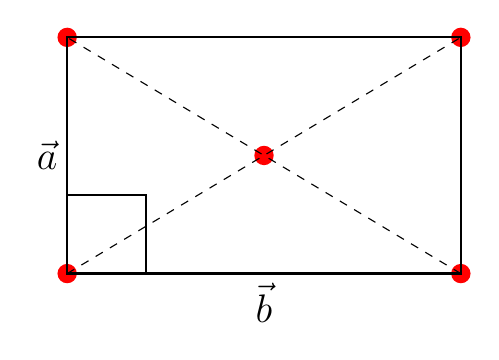
\begin{tikzpicture}
    \def\a{5}  % length of side a
    \def\b{3}  % length of side b

    % Calculate the coordinates of the points
    \coordinate (A) at (0, 0);
    \coordinate (B) at (\a, 0);
    \coordinate (C) at (\a, \b);
    \coordinate (D) at (0, \b);
    %\coordinate (E) at (\a, 2*\b);
    %\coordinate (F) at (0, 2*\b);

    % Creates node labels
    %\node[above left] at (A) {A};
    %\node[above left] at (B) {B};
    %\node[above left] at (C) {C};
    %\node[above left] at (D) {D};
    %\node[above left] at (E) {E};
    %\node[above left] at (F) {F};

    % Creates nodes at vertices
    \fill[red]  (A) circle(3.5pt) (B) circle(3.5pt) (C) circle(3.5pt) (D) circle(3.5pt);% (E) circle(3.5pt) (F) circle(3.5pt);
    % Creates nodes at centers
    \fill[red] ($(A)!0.5!(C)$) circle(3.5pt);
    %\fill[blue] ($(D)!0.5!(E)$) circle(3.5pt);

    % Draw the rectangular unit cell
    \draw[thick] (A) -- (B) -- (C) -- (D) -- cycle;
    %\draw[thick,dashed] (D) -- (F) -- (E) -- (C) -- cycle;
    %\draw[thick] (D) -- ($(A)!0.5!(C)$) -- (C) -- ($(D)!0.5!(E)$) -- cycle;

    % Draw lines
    \draw[dashed] (A) -- (C);
    \draw[dashed] (B) -- (D);

    % Draw right angle
    \draw[thick] (0,1) -- (1,1) -- (1,0);


    %Draw lattice parameters
    \node[left] at ($(A)!0.5!(D)$) {\Large $\vec{a}$};
    \node[below] at ($(A)!0.5!(B)$) {\Large $\vec{b}$};
    
\end{tikzpicture}

\end{document}